%%%%%%%%%%%%%%%%%%%%%%%%%%%%%%%%%%%%%%%%%
% CSE 4316/4317 Sprint Report Template
% Version 1.0 (2/18/2018)
% Author: Christopher D. McMurrough
%%%%%%%%%%%%%%%%%%%%%%%%%%%%%%%%%%%%%%%%%

%----------------------------------------------------------------------------------------
%	PACKAGES AND DOCUMENT CONFIGURATIONS
%----------------------------------------------------------------------------------------

\documentclass{article}
\usepackage{siunitx}
\usepackage{graphicx}
\usepackage{amsmath}
\setlength\parindent{0pt}

\usepackage[letterpaper, portrait, margin=1in]{geometry}

%----------------------------------------------------------------------------------------
%	DOCUMENT SECTIONS
%----------------------------------------------------------------------------------------

% report title
\title{Sprint 1 Report \\ CSE 4316}

% author name
\author{Atafo Abure}

% date of assignment submission
\date{Thursday 3rd, 2019}

\begin{document}
\maketitle
\begin{center}
\begin{tabular}{l r}

% sprint start date
Sprint start date: & September 14th, 2019 \\

% sprint end date
Sprint end date: & October 1st, 2019 \\

% project title
Project title: & Smart Shutters \\

% team name
Team name: & No SHUT Eye \\

% team members
Partners: 	& Haris Qureshi\\
			& David Nquyen\\
			& Deion Nwaefulu \\
        	& Aditya Rajguru \\
Instructor: & Shawn Gieser
\end{tabular}
\end{center}

% sprint goal
\section{Sprint Goal}
Requirements Elicitation and Completion of Project Charter

% sprint backlog
\section{Sprint Backlog}
Breakdown of planned tasks assigned to team (work units expressed in hours) \\ % work units do not have to be hours, change text accordingly

% ADD OR REMOVE ROWS FROM THE TABLE AS NECESSARY (DO NOT LEAVE BLANK ROWS!)
\begin{tabular}{| p{4in} | >{\centering\arraybackslash} p{1in} | >{\centering\arraybackslash} p{1in} |}
\hline
TASK DESCRIPTION & ESTIMATED WORK & ACTUAL WORK \\ \hline
Review LaTex & 24 & 12 \\ \hline
Project Charter Initial Draft & 96 & 96 \\ \hline
Review Initial Draft & 12 & 6 \\ \hline
Write Final Draft & 12 & 12 \\ \hline
Review Final Draft & 12 & 12 \\ \hline
Brainstorming & 60 & 36 \\ \hline
Document Analysis & 36 & 12 \\ \hline
Hardware Details & 240 & 24 \\ \hline
High Level System Architecture & 672 & 12 \\ \hline
Process Modeling & 60 & 24 \\ \hline
\textbf{TOTAL} & \textbf{720}  & \textbf{246} \\ \hline
\end{tabular}

\pagebreak

% individual time summary
\section{Individual Time Expenditures}
Summary of tasks performed by the individual (work units expressed in hours) \\ % work units do not have to be hours, change text accordingly

% ADD OR REMOVE ROWS FROM THE TABLE AS NECESSARY (DO NOT LEAVE BLANK ROWS!)
% PERCENT COMPLETE DESCRIBES THE STATE OF THE TASK AS OF THE LAST SPRINT DAY (WAS IT FINISHED? IF NOT, APPROXIMATELY HOW "COMPLETE" IS THE TASK)
\begin{tabular}{| p{4in} | >{\centering\arraybackslash} p{1in} | >{\centering\arraybackslash} p{1in} |}
\hline
TASK DESCRIPTION & ACTUAL WORK & PERCENT COMPLETE \\ \hline
Project Charter Initial Draft & 96 & 100\% \\ \hline
Write Final Draft & 12 & 100\% \\ \hline
Brainstorming & 36 & 25\% \\ \hline
Document Analysis & 12 & 100\% \\ \hline
High Level System Architecture & 12 & 10\% \\ \hline
\textbf{TOTAL} & \textbf{5.0}  & \textbf{-} \\ \hline
\end{tabular}

% burndown chart
\section{Team Burndown Chart}
Burndown chart showing day-to-day progress on sprint tasks. Ideal (baseline) daily effort and actual daily effort of the team are both shown in the figure below.
\begin{figure}[h]
\begin{center}
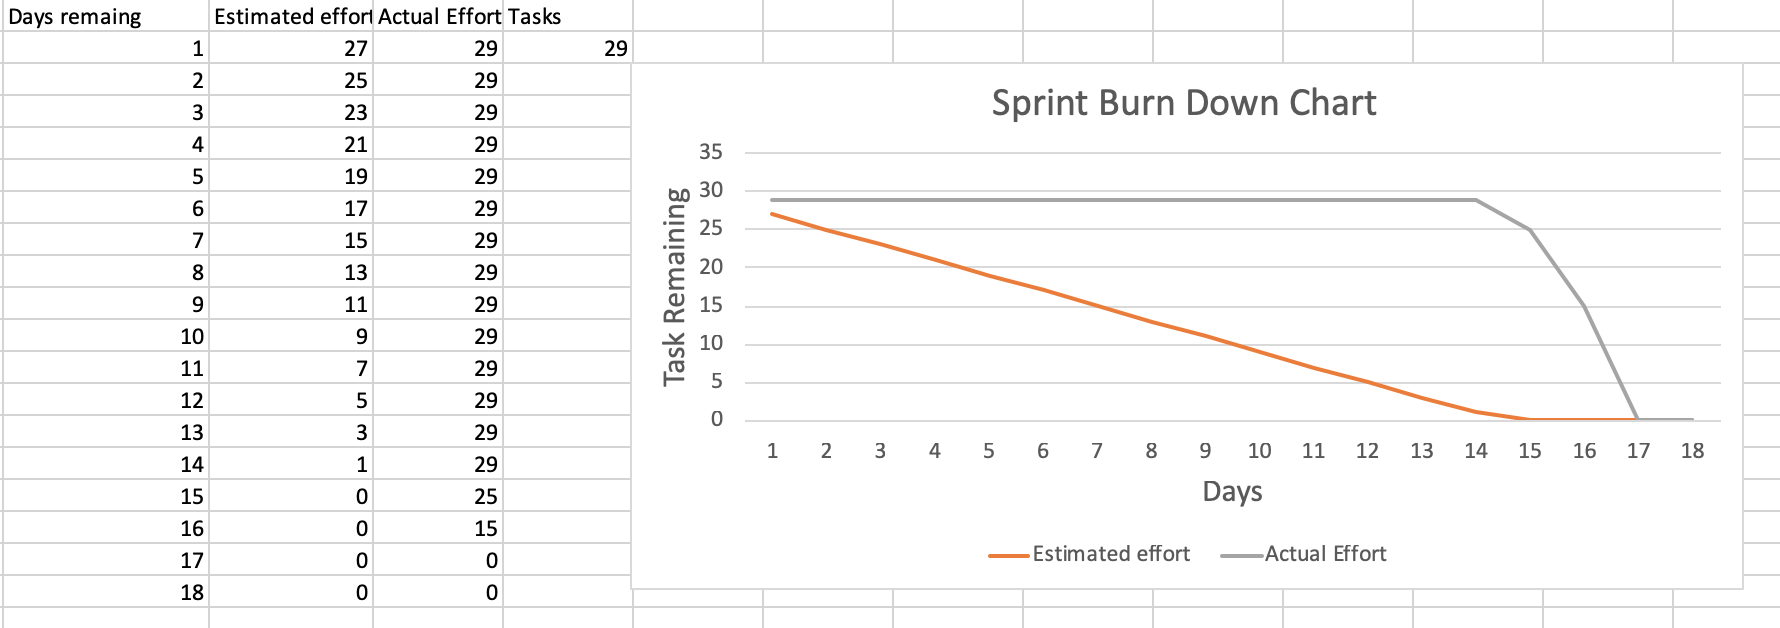
\includegraphics[width=1.0\textwidth]{SprintBurn} % Include the image burndown.png
\end{center}
\end{figure}

\pagebreak

%individual sprint retrospective
\section{Individual Retrospective}
The following lists describe actions (as an individual) that will be started, stopped, or continued during the next sprint to maximize work efficiency. \\

Actions and/or items to \textbf{start} doing in the next sprint (top 3)
\begin{itemize}
\begin{item}
Description of first item
\end{item}
\begin{item}
Description of second item
\end{item}
\begin{item}
Description of third item
\end{item}
\end{itemize}

Actions and/or items to \textbf{stop} doing in the next sprint (top 3)
\begin{itemize}
\begin{item}
Description of first item
\end{item}
\begin{item}
Description of second item
\end{item}
\begin{item}
Description of third item
\end{item}
\end{itemize}

Actions and/or items to \textbf{continue} doing in the next sprint (top 3)
\begin{itemize}
\begin{item}
Description of first item
\end{item}
\begin{item}
Description of second item
\end{item}
\begin{item}
Description of third item
\end{item}
\end{itemize}

\end{document}